\documentclass[tikz,border=5pt]{standalone}
\usepackage{tikz}
\usetikzlibrary{trees}
\usetikzlibrary{patterns}

\begin{document}

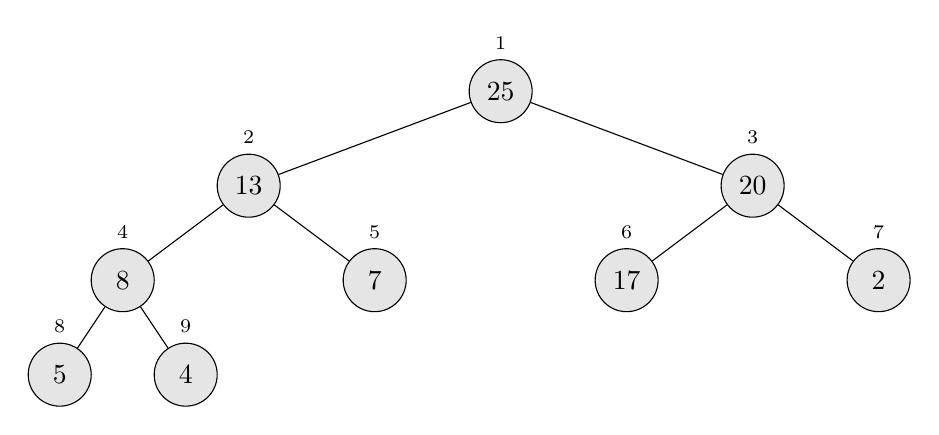
\begin{tikzpicture}[
  level distance=12mm,
  % every node/.style={circle, draw, minimum size=2mm},
  level 1/.style={sibling distance=64mm},
  level 2/.style={sibling distance=32mm},
  level 3/.style={sibling distance=16mm},
  level 4/.style={sibling distance=8mm},
    treenode/.style={
    draw,
    circle,
    minimum size=8mm,
    inner sep=0pt,
    fill=gray!20,
    font=\normalsize
  },
  orphan/.style={
    edge from parent/.style={draw=none}
  },
  orphannode/.style={
    treenode,
    fill=gray!70,
    font=\bfseries
  },
  every label/.style={font=\scriptsize}
]

% For illustrating heap
\node[treenode,label=above:1]{25}
  child { node[treenode,label=above:2]{13}
    child { node[treenode,label=above:4]{8}
      child { node[treenode,label=above:8]{5}}
      child { node[treenode,label=above:9]{4}}
    }
    child { node[treenode,label=above:5]{7}
      % child { node[treenode,label=above:10]{12}}
      % child { node[treenode,label=above:11]{4}}
    }
  }
  child { node[treenode,label=above:3]{20}
    child { node[treenode,label=above:6]{17} 
      % child { node[treenode,label=above:12]{8}}
      % child { node[treenode,label=above:13]{3}}
    }
    child { node[treenode,label=above:7]{2}
      % child { node[treenode,label=above:14]{0}}
      % child[missing]
    }
  };

% For illustrating heapsort
% \node[treenode,label=above:1]{13}
%   child { node[treenode,label=above:2]{8}
%     child { node[treenode,label=above:4]{2}
%       child[orphan] { node[orphannode,label=above:8]{20}}
%       child[orphan] { node[orphannode,label=above:9]{25}}
%     }
%     child { node[treenode,label=above:5]{7}}
%   }
%   child { node[treenode,label=above:3]{5}
%     child { node[treenode,label=above:6]{4}}
%     child[orphan] { node[orphannode,label=above:7]{17}}
%   };
\end{tikzpicture}

% ,label=right:\textit{i},fill=gray!60
% ,pattern=crosshatch,pattern color=gray!60

\end{document}
